\section{Sample section}
This is sample text.
此れは標本文章である。
参考文献テスト\cite{Sample2000}。参考文献テスト\cite{discovery, Laskar}。

% theorem
\begin{SampleA}
    サンプル用定理環境A。
\end{SampleA}
\begin{SampleB}
    サンプル用定理環境B(番号がSampleAに従う)。
\end{SampleB}
\begin{SampleC}
    サンプル用定理環境C(番号なし)。
\end{SampleC}

% fonts
Table \ref{sample_font} is sample font.
\begin{table}
    \centering
    \caption{Sample font(style)}
    \begin{tabular}{|c|c|c|}
        \hline
        style & description & appearance \\ \hline
        normal & -- & Sample text \\ \hline
        bold & \texttt{\textbackslash textbf\{\}} & \textbf{Sample text. 標本文章。} \\ \hline
        emphasise & \texttt{\textbackslash emph\{\}} & \emph{Sample text. 標本文章。} \\ \hline
        italic & \texttt{\textbackslash textit\{\}} & \textit{Sample text. 標本文章。} \\ \hline
        default weight & \texttt{\textbackslash textmd\{\}} & \textmd{Sample text. 標本文章。} \\ \hline
        small capital & \texttt{\textbackslash textsc\{\}} & \textsc{Sample text. 標本文章。} \\ \hline
        sans serif & \texttt{\textbackslash textsf\{\}} & \textsf{Sample text. 標本文章。} \\ \hline
        slant & \texttt{\textbackslash textsl\{\}} & \textsl{Sample text. 標本文章。} \\ \hline
        typewriter & \texttt{\textbackslash texttt\{\}} & \texttt{Sample text. 標本文章。} \\ \hline
        upshape & \texttt{\textbackslash textup\{\}} & \textup{Sample text. 標本文章。} \\ \hline
    \end{tabular}
    \label{sample_font}
\end{table}

% figure
Figure \ref{sample_figure} is sample figure.
\begin{figure}
    \centering
    \subfigure[Sheep(PNG)]{
\includegraphics[width=4cm]{figures/sample_imgs/sheep.png}}
    \subfigure[Lion(JPG)]{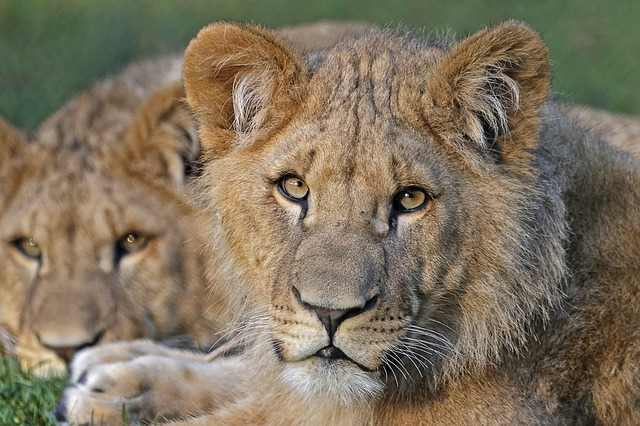
\includegraphics[width=4cm]{figures/sample_imgs/lion.jpg}}
    \subfigure[Boy(PDF)]{
\includegraphics[width=4cm]{figures/sample_imgs/boy.pdf}}
    \caption{Sample figures}
    \label{sample_figure}
\end{figure}

% table
Table \ref{sample_table} is sample table.
\begin{table}
    \centering
    \caption{Sample table}
    \begin{tabular}{|c|c|c|c|}
        \hline
        \multirow{2}{*}{Sample-A} & \multicolumn{3}{|c|}{Sample-B} \\ \cline{2-4}
        & Sample-C & Sample-D & Sample-E \\ \hline
        \multirow{3}{*}{Sample-F} & Sample-G & Sample-H & Sample-I \\ \cline{2-4}
        & \multirow{2}{*}{Sample-J} & \multicolumn{2}{|c|}{Sample-K} \\ \cline{3-4}
        & & Sample-L & Sample-M \\ \hline
    \end{tabular}
    \label{sample_table}
\end{table}

% listing
List \ref{sample_list1} and \ref{sample_list2} is sample code.

\begin{code}
    \caption{Sample code 1}
    \lstinputlisting[language=Python]{input/sample_code.py}
    \label{sample_list1}
\end{code}

\begin{code*}
    \caption{Sample code 2}
    \lstinputlisting[language=Python]{input/sample_code.py}
    \label{sample_list2}
\end{code*}

